%!TEX program = xelatex
\documentclass{beamer}
%!TEX root = P_Manual.tex
\usepackage[spanish]{babel}

\usepackage{graphicx,hyperref,url, materialbeamer}
\usepackage{braket}
%\usepackage{euler}
\usepackage{listings}
\usepackage{booktabs}% to use \toprule
\usepackage{xfrac}% to use \sfrac{}{}

\graphicspath{ {./figs/} }
\setbeamercovered{transparent}
\lstdefinestyle{customc}{
  belowcaptionskip=1\baselineskip,
  breaklines=true,
  xleftmargin=\parindent,
  language=C,
  showstringspaces=false,
  basicstyle=\footnotesize\ttfamily,
  keywordstyle=\bfseries\color{green!40!black},
  commentstyle=\itshape\color{purple!40!black},
  identifierstyle=\color{blue},
  stringstyle=\color{orange},
  extendedchars=true,
  breakatwhitespace=false
}
\lstset{escapechar=@,style=customc}



\usefonttheme{professionalfonts} % using non standard fonts for beamer
%\usefonttheme{serif}

% The title of the presentation:
%  - first a short version which is visible at the bottom of each slide;
%  - second the full title shown on the title slide;
\title[Programación]{Programación}

% Optional: a subtitle to be dispalyed on the title slide
\subtitle{Tronco Común de Ingeniería \\ FCQI}

% The author(s) of the presentation:
%  - again first a short version to be displayed at the bottom;
%  - next the full list of authors, which may include contact information;
\author[Violeta Ocegueda]{Violeta Ocegueda} 
  
%\titlegraphic{\includegraphics[width=\textwidth]{atac-logo}}

% The institute:
%  - to start the name of the university as displayed on the top of each slide
%    this can be adjusted such that you can also create a Dutch version
%  - next the institute information as displayed on the title slide
\institute[UABC]{Profesor-Investigador \\ Facultad de Ciencias Químicas e Ingeniería \\ Universidad Autónoma de Baja California \\ Campus Tijuana}

% Add a date and possibly the name of the event to the slides
%  - again first a short version to be shown at the bottom of each slide
%  - second the full date and event name for the title slide
\date[\today]{\today}

\providecommand{\di}{\mathop{}\!\mathrm{d}}
\providecommand*{\der}[3][]{\frac{d\if?#1?\else^{#1}\fi#2}{d #3\if?#1?\else^{#1}\fi}} 
 \providecommand*{\pder}[3][]{% 
    \frac{\partial\if?#1?\else^{#1}\fi#2}{\partial #3\if?#1?\else^{#1}\fi}% 
  }

\begin{document}
	%!TEX root = P_Manual.tex
\begin{frame}
  	\titlepage
\end{frame}

\begin{frame}{Contenido}
	\tableofcontents
\end{frame}
	\setlength{\parskip}{\baselineskip} 
\section{Metodología}

\begin{frame}[c] 
\frametitle{}
\centering
\huge \textbf{Metodología para la resolución de problemas}
\end{frame}

\begin{frame}[t]
\frametitle{Metodología para la resolución de problemas}
\begin{block}{\textbf{Problema}}
Un problema se entiende como una proposición que, a partir de ciertas condiciones conocidas, induce a buscar algo desconocido.
\end{block}
El proceso de resolución de un problema con una computadora conduce a la escritura de un programa y a su ejecución en la misma. Aunque el proceso de diseñar programas es -esencialmente- un \textbf{proceso creativo}, se pueden considerar una serie de fases o pasos comunes a seguir.
\end{frame}

\begin{frame}[t]
\frametitle{Metodología para la resolución de problemas}
Las fases de resolución de un problema con computadora son:
\begin{itemize}
    \item Análisis del problema \pause
    \item Diseño del algoritmo \pause
    \item Codificación \pause
    \item Compilación y ejecución \pause
    \item Verificación \pause
    \item Depuración \pause
    \item Mantenimiento \pause
    \item Documentación
\end{itemize}
\end{frame}

\begin{frame}[t]
\frametitle{Análisis del problema}
\begin{itemize}
    \item Es la primera fase de la resolución de un problema con computadora.
    \item Requiere una clara definición de las \textbf{entradas} y \textbf{salidas}.
\end{itemize}
\textbf{Ejercicio:} Describa el proceso de retirar dinero del cajero.
\end{frame}

\begin{frame}[t]
\frametitle{Diseño del algoritmo}
\begin{block}{\textbf{Algoritmo}}
Un algoritmo es un \textcolor{orange}{conjunto de pasos}, procedimientos o acciones que nos permiten alcanzar un resultado o \textcolor{orange}{resolver un problema}.
\end{block}
Un algoritmo se puede concebir como un \textcolor{orange}{diálogo entre una computadora y una persona}, en el que se especifica bajo qué condiciones la computadora debe generar la salida específica.
\end{frame}

\begin{frame}[t]
\frametitle{Características de los algoritmos}
Las características que los algoritmos deben reunir son las siguientes:
\begin{itemize}
    \item \textcolor{blue}{Precisión:} los pasos a seguir en el algoritmo deben ser precisados claramente. \pause
    \item \textcolor{blue}{Determinismo:} dado un conjunto de datos idénticos de entrada, siempre debe arrojar los mismos resultados. \pause
    \item \textcolor{blue}{Finitud:} independientemente de su complejidad, siempre debe ser de longitud finita. 
\end{itemize}
\end{frame}

\begin{frame}[t]
\frametitle{Diagrama de flujo}
Un \textcolor{blue}{diagrama de flujo} representa la \textcolor{orange}{esquematización gráfica} de un algoritmo. Es decir, muestra gráficamente los pasos o procesos a seguir para alcanzar la \textcolor{orange}{solución de un problema}.
\end{frame}

\begin{frame}[t]
\frametitle{Símbolos utilizados en los diagramas de flujo}
\begin{center}
    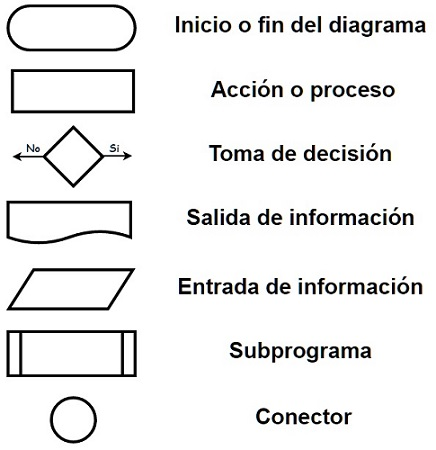
\includegraphics[width=0.57\textwidth]{figs/diagrama_flujo_simbolos}
\end{center}
\end{frame}

\begin{frame}[t]
\frametitle{Codificación}
\textcolor{blue}{Codificación} es la escritura en un lenguaje de programación de la representación del algoritmo desarrollada en etapas anteriores.
\end{frame}

\begin{frame}[t]
\frametitle{Depuración}
La \textcolor{blue}{depuración} es el proceso de encontrar los errores del programa y corregir o eliminar dichos errores.\\
Cuando se ejecuta un programa se pueden producir tres tipos de errores:
\begin{itemize}
    \item \textcolor{blue}{Errores de compilación:} o \textit{errores de sintaxis}, se producen normalmente por un uso incorrecto de las reglas del lenguaje de programación. \pause
    \item \textcolor{blue}{Errores de ejecución:} se producen por instrucciones que la computadora puede comprender pero no ejecutar (división por cero, raíces cuadradas de números negativos). \pause
    \item \textcolor{blue}{Errores lógicos:} se producen en la lógica del programa y la fuente del error suele ser el diseño del algoritmo.
\end{itemize}
\end{frame}


\begin{frame}[t]
\frametitle{Ejercicios}
Realiza el análisis, el algoritmo y el diagrama de flujo de los siguiente problemas:
\begin{itemize}
    \item Calcular la suma de dos números.
    \item Calcular el área de un triángulo.
    \item Calcular la hipotenusa de un triángulo.
    \item Identificar el mayor de dos números.
    \item Identificar el mayor de tres números.
    \item Imprimir los primeros diez números pares.
\end{itemize}
\end{frame}



%\begin{frame}
%\frametitle{Before Tao}
%	\begin{itemize}
% 	\item Facebook was storing the social graph to MySql
%	\begin{itemize}
%		\item  	Quering it from PHP
%		\item  	Storing result in memcache\\
%	\end{itemize}
%	\end{itemize}
%	\begin{center}
%		\includegraphics[width=0.3\textwidth]{figs/php-logo.eps}\quad
%		\includegraphics[width=0.3\textwidth]{figs/mysql.png}
%	\end{center}
% 	Over time Fb deprecated direct access to MySQL in favor of a graph (associations, nodes) abstraction
%\end{frame}




	%!TEX root = P_Manual.tex
\setlength{\parskip}{\baselineskip} 
\section{Lenguaje}

% ----------------------- Slide 01-------------------------------- %
\begin{frame}[c] 
\frametitle{}
\centering
\huge \textbf{Introducción al lenguaje de programación}
\end{frame}


% --------------------------- Slide 02 ---------------------------------- %
\begin{frame}[t, fragile]{Estructura básica de un programa}
%	\frametitle{Estructura básica de un programa}
	\begin{lstlisting}
/* Inclusion de librerias */

void main() /* cabecera de funcion */
{ /* inicio de la funcion main */

... /* Sentencias */

} /* fin de la funcion main */
\end{lstlisting}
\end{frame}


% ------------------------- Slide 03 --------------------------------- %
\begin{frame}[fragile]{Estructura básica de un programa para la clase}
%	\frametitle{Estructura básica de un programa para la clase}
	\begin{lstlisting}
/* Inclusion de librerias */

void main() /* cabecera de funcion */
{ /* inicio de la funcion main */

/* Declaracion de variables */

/* Entrada de datos */

/* Procesamiento */

/* Impresion de resultados */

} /* fin de la funcion main */
\end{lstlisting}
\end{frame}


% -------------------------- Slide 04 ---------------------------------- %
\begin{frame}[fragile, t]{Zonas de memoria}
%	\frametitle{Zonas de memoria}
	\textbf{Variables}\\
	\footnotesize
	\begin{itemize}
		\item Son objetos que pueden cambiar su valor durante la ejecución de un programa.
		\item En C una \textit{variable} es una posición en memoria con nombre donde se almacena un valor de un cierto tipo de dato.
	\end{itemize}
	\vspace{-2mm}
	La \textit{declaración} de una variable es una sentencia que proporciona información de la variable al compilador C. Su sintaxis es:
	\begin{lstlisting}
<tipo_variable> <nombre_variable> = <valor_inicial>;
\end{lstlisting}
	\vspace{-4mm}
	Donde:
	\vspace{-4mm}
	\begin{itemize}
		\item \textit{tipo\_variable} es el nombre de un tipo de dato conocido por C.
		\item \textit{nombre\_variable} es un identificador (nombre) válido en C.
		\item \textit{valor\_inicial} es el valor de inicialización de la variable.
	\end{itemize}
\end{frame}

% --------------------------- Slide 05 --------------------------------- %
\begin{frame}[t, fragile]{Zonas de memoria}
	%\frametitle{Zonas de memoria}
	\textbf{Tipos de datos}\\
	\footnotesize
	Los tipos de datos básicos son:
	\begin{itemize}
		\item enteros
		\item flotantes
		\item caracteres
	\end{itemize}
	\textbf{Constantes}\\
	Las \textit{constantes} son datos que no cambian durante la ejecución de un programa.
	\begin{lstlisting}
#define NUEVALINEA \n 
#define PI 3.141592 
#define VALOR 54
\end{lstlisting}
\end{frame}


% --------------------------- Slide 06 --------------------------------- %
\begin{frame}[t]{Operadores}
\textbf{Operadores de asignación y expresión}\\
\begin{center}
	\begin{tabular}{ccc}
		\toprule
		\textbf{Operador} & \textbf{Expresión} & \textbf{Explicación} \\
		\midrule
		+= & c += 7 & c = c + 7 \\ \hline
		-= & d -= 4 & d = d - 4 \\ \hline
		*= & e *= 5 & e = e * 5 \\ \hline
		/= & f/= 3 & f = f / 3 \\ \hline
		\hspace{1mm} \%= & g \%= 9 & g = g \% 9 \\
		\bottomrule
	\end{tabular}
\end{center}
\end{frame}

% --------------------------- Slide 07 --------------------------------- %
\begin{frame}[t]{Operadores}
\textbf{Operadores aritméticos}\\
\vspace{5mm}
\small
\begin{center}
	\begin{tabular}{cccc}
		\toprule
		\textbf{Operador} & \textbf{Operación} & \textbf{Expresión algebraica} & \textbf{Expresión en C}\\
		\midrule
		+ & Suma & f + 7 & f + 7 \\ \hline
		- & Resta & p - c & p - c\\ \hline
		* & Multiplicación & bm & b * m\\ \hline
		/ & División & $\frac{x}{y}$ ó $\sfrac{x}{y}$ & x / y \\ \hline
	\end{tabular}
\end{center}
\end{frame}

% --------------------------- Slide 08 --------------------------------- %
\begin{frame}[t]{Operadores}
\textbf{Operadores de relación}\\ \vspace{5mm}
\begin{center}
\begin{tabular}{ccl}
	\toprule
	\textbf{Operador} & \textbf{Ejemplo} & \textbf{Significado}\\
	\midrule
	== & x == y & x es igual que y \\ \hline
	!= & x != y & x es diferente de y \\ \hline
	> & x > y & x es mayor que y \\ \hline
	< & x < y & x es menor que y \\ \hline
	>= & x >= y & x es mayor o igual que y \\ \hline
	<= & x <= y & x es menos o igual que y \\ 
	\bottomrule
\end{tabular}
\end{center}
\end{frame}

% --------------------------- Slide 09 --------------------------------- %
\begin{frame}[t]{Operadores}
\textbf{Operadores lógicos: AND lógico}\\ \vspace{3mm}
\small
\begin{center}
%\caption{Tabla de verdad para el operador \textit{\&\&} (AND l\'ogico).}
\begin{tabular}{llc}
	\toprule
	\textbf{expresión} & \textbf{expresión2} & \textbf{expresión1 \&\& expresión2}\\
	\midrule \hline
	0 & 0 & 0 \\
	0 & diferente de cero & 0\\
	diferente de cero & 0 & 0\\
	diferente de cero & diferente de cero & 1\\ \hline
	\bottomrule
\end{tabular}
\end{center}
\end{frame}

% --------------------------- Slide 10 ------------------------------ %
\begin{frame}[t]{Operadores}
\textbf{Operadores lógicos: OR lógico}\\ \vspace{5mm}
\centering
%\caption{Tabla de verdad para el operador \textit{| |} (OR l\'ogico).}
\begin{tabular}{llc}
	\toprule
	\textbf{expresión1} & \textbf{expresión2} & \textbf{expresión1 $| |$ expresión2}\\
	\midrule \hline
	0 & 0 & 0 \\
	0 & diferente de cero & 1\\
	diferente de cero & 0 & 1\\
	diferente de cero & diferente de cero & 1\\ \hline
	\bottomrule
\end{tabular}
\end{frame}

% --------------------------- Slide 11 --------------------------------- %
\begin{frame}[t]
\frametitle{Operadores}
\textbf{Operadores lógicos: NOT lógico}\\ \vspace{5mm}
\centering
%\caption{Tabla de verdad para el operador \textbf{!} (negaci\'on l\'ogico).}
\begin{tabular}{lc}
\toprule
\textbf{expresión} & \textbf{!expresión}\\
\midrule \hline
0 & 1 \\
diferente de cero & 0\\
\bottomrule
\end{tabular}
\end{frame}

% --------------------------- Slide 12 --------------------------------- %
\begin{frame}[t]{Operadores}
\textbf{Operadores de incremento y decremento}\\ \vspace{5mm}
\footnotesize
\begin{center}
%\caption{Operadores de incremento y decremento}
\begin{tabular}{ccp{7.5cm}}
	\toprule
	\textbf{Operador} & \textbf{Ejemplo} & \textbf{Explicación}\\
	\midrule
	++&++a& Incrementar a en 1 y después utiliza el nuevo valor de a en la expresión en la que reside.\\
	++ & a++ & Utiliza el valor actual de a en la expresión en la que reside, y después la incrementa en 1.\\
	$--$ & $--$b & Decrementar b en 1 y después utiliza el nuevo valor de b en la expresión en la que reside.\\
	$--$ & b$--$ & Utiliza el valor actual de b en la expresión en la que reside, y después decrementa b en 1.\\
	\bottomrule
\end{tabular}
\end{center}
\end{frame}


% --------------------------- Slide 13 --------------------------------- %
\begin{frame}[t]{Operadores}
\textbf{Jerarquía de operadores}\\ \vspace{5mm}
\scriptsize
%\begin{table}[h]
\centering
%\caption{Jerarqu\'ia de operadores}
\begin{tabular}{ccll}
	\toprule
	\textbf{Jerarqu\'ia} & \textbf{Operadores} & \textbf{Asociatividad} & \textbf{Tipo}\\ 
	\midrule 
	Mayor & $++$ $--$ $+$ $-$ $!$ & derecha a izquierda & unario\\ \cline{2-4}
	| & * / \% & izquierda a derecha & multiplicativo\\ \cline{2-4}
	| & + $-$ & izquierda a derecha & aditivo\\ \cline{2-4}
	| & $<$ $<=$ $>$ $>=$ & izquierda a derecha & de relaci\'on \\ \cline{2-4}
	| & == != & izquierda a derecha & de relación\\ \cline{2-4}
	| & \&\& & izquierda a derecha & AND lógico\\ \cline{2-4}
	| & $| |$ & izquierda a derecha & OR lógico \\ \cline{2-4}
	Menor & $=$, $+=$, $-=$, $*=$, $/=$, $\%=$ & derecha a izquierda & de asignación \\ 
	\bottomrule
\end{tabular}
%\end{table}
\end{frame}


% --------------------------- Slide 14 --------------------------------- %
\begin{frame}{Instrucción de salida}
La instrucción de salida utilizada en C se denomina \textbf{printf}. Su sintaxis es:\\
\vspace{5mm}

{\small \textit{printf( ``texto a imprimir'' );}\\
\textit{printf( ``texto a imprimir \%formato\_de\_impresión'',variable\_a\_imprimir );}}
\end{frame}


% --------------------------- Slide 15 --------------------------------- %
\begin{frame}[t]
\frametitle{Formato de salida con printf}
\textbf{Especificadores de conversión entera para \textit{printf}}\\ \vspace{5mm}
\scriptsize
%\begin{table}[h]
\begin{center}
%\caption{Especificadores de conversi\'on entera para \textit{printf}}
\begin{tabular}{lp{7.5cm}}
	\toprule
	\textbf{Especificador} & \textbf{Descripción}\\
	\midrule
	\textbf{\%d} & Despliega un entero decimal con signo.\\ 
	\textbf{\%i} & Despliega un entero decimal con signo. [Nota: los especificadores i y d son diferentes cuando se utilizan con \textbf{scanf}.]\\ 
	\textbf{\%o} & Despliega un entero octal sin signo.\\
	\textbf{\%u} & Despliega un entero decimal sin signo. \\
	\textbf{\%x} ó \textbf{\%X} & Despliega un entero hexadecimal sin signo. \textbf{X} provoca que se desplieguen los dígitos de \textbf{0} a \textbf{9} y las letras de \textbf{A} a \textbf{F}, y \textbf{x} provoca que se desplieguen los dígitos de \textbf{0} a \textbf{9} y las letras de \textbf{a} a \textbf{f}.\\ 
	\textbf{h} ó \textbf{l} (letra l) & Se coloca antes de cualquier especificador de conversión entera para indicar que se despliega un entero corto o largo, respectivamente. Las letras \textbf{h} y \textbf{l} son llamadas con más precisión \textit{modificadores de longitud}.\\
	\bottomrule
\end{tabular}
%\end{table}
\end{center}
\end{frame}
% --------------------------- Slide 16 --------------------------------- %
\begin{frame}[t]{Formato de salida con printf}
\textbf{Especificadores de conversi\'on de punto flotante para \textit{printf}}\\ \vspace{5mm}
\scriptsize
\centering
%\caption{Especificadores de conversi\'on de punto flotante para \textit{printf}}
\begin{tabular}{lp{7.5cm}}
	\toprule
	\textbf{Especificador} & \textbf{Descripción}\\
	\midrule 
	\textbf{\%e} \'o \textbf{\%E} & Despliega un valor de punto flotante con notaci\'on exponencial.\\
	\textbf{\%f} & Despliega un valor de punto flotante con notaci\'on de punto fijo.\\
	\textbf{\%g} \'o \textbf{\%G} & Despliega un valor de punto flotante con el formato de punto flotante \textbf{f}, o con el formato exponencial \textbf{e} (o \textbf{E}) basado en la magnitud del valor. \\
	\textbf{L} & Se coloca antes del especificador de conversión para indicar que se desplegar\'a un valor de punto flotante \textbf{long double}\\ 
	\bottomrule
\end{tabular}
\end{frame}

% --------------------------- Slide 17 --------------------------------- %
\begin{frame}[t]{Formato de salida con printf}
\textbf{Especificadores de conversión de caracteres y cadenas para \textit{printf}}\\ \vspace{5mm}
%\scriptsize
\centering
%\caption{Especificadores de conversi\'on de caracteres y cadenas para \textit{printf}}
\begin{tabular}{lp{7.5cm}}
	\toprule
	\textbf{Especificador} & \textbf{Descripci\'on}\\
	\midrule
	\textbf{\%c} & Despliega caracteres individuales.\\
	\textbf{\%s} & Despliega cadenas de caracteres. \\
	\bottomrule
\end{tabular}
\end{frame}

% --------------------------- Slide 18 --------------------------------- %
\begin{frame}[t]{Formato de salida con printf}
\textbf{Otros especificadores de conversi\'on para \textit{printf}}\\ \vspace{5mm}
\scriptsize
\begin{center}
%\caption{Otros especificadores de conversi\'on para \textit{printf}}
\begin{tabular}{lp{7.5cm}}
	\toprule
	\textbf{Especificador} & \textbf{Descripción}\\
	\midrule
	\textbf{\%p} & Despliega un valor apuntador de manera definida por la implementación.\\ 
	\textbf{\%n} & Almacena el número de caracteres ya desplegados en la instrucci\'on \textbf{printf} actual. Proporciona un apuntador a un entero como el argumento correspondiente. No despliega valor alguno.\\ 
	\textbf{\%\%} & Despliega el caracter de porcentaje.\\
	\bottomrule
\end{tabular}
\end{center}
\end{frame}

% --------------------------- Slide 19 --------------------------------- %
\begin{frame}[t]{Secuencias de escape}
\small
\begin{center}
\begin{tabular}{p{3.5cm}p{6.5cm}}
	\toprule
	\textbf{Secuencia de escape} & \textbf{Descripción}\\
	\midrule
	\textbackslash a (alerta o campana) & Provoca una alerta sonora (campana) o una alerta visual.\\
	\textbackslash \textbackslash (diagonal invertida) & Despliega el caracter de diagonal invertida (\textbackslash).\\
	\textbackslash ' (comilla sencilla) & Despliega el caracter de comilla sencilla (').
	\\
	\textbackslash '' (comilla doble) & Despliega el caracter de comilla doble (''). \\ 
	\textbackslash ? (interrogación) & Despliega el caracter de interrogación (?).\\
	\textbackslash n (nueva línea) & Mueve el cursor al inicio de la siguiente línea.\\
	\bottomrule
\end{tabular}
\end{center}
\end{frame}

% --------------------------- Slide 20 --------------------------------- %
\begin{frame}[t]{Secuencias de escape (Continuación)}
\vspace{-4mm}
\small
\begin{center}
	\begin{tabular}{p{4cm}p{6cm}}
		\toprule
		\textbf{Secuencia de escape} & \textbf{Descripción}\\
		\midrule 
		\textbackslash t (tabulador horizontal) & Mueve el cursor a la siguiente posición del tabulador.\\
		\textbackslash b (retroceso) & Mueve el cursor una posición hacia atrás en la línea actual.\\
		\textbackslash f (nueva página o avance de página) & Mueve el cursor al inicio de la siguiente página l\'ogica.\\
		\textbackslash r (retorno de carro) & Mueve el cursor al principio de la línea actual.\\
		\textbackslash v (tabulador vertical) & Mueve el cursor a la siguiente posición del tabulador vertical.\\
		\bottomrule
	\end{tabular}
\end{center}
\end{frame}

% --------------------------- Slide 21 --------------------------------- %
\begin{frame}{Banderas de la cadena de control de formato}
\small
%\begin{table}[h]
\centering
%\caption{Banderas de la cadena de control de formato}
\begin{tabular}{lp{6cm}}
	\toprule
	\textbf{Bandera} & \textbf{Descripción}\\
	\midrule 
	\textbackslash$-$ (signo menos) & Justifica la salida a la izquierda dentro del campo especificado.\\ 
	\hline
	\textbackslash+ (signo más) & Despliega el signo más que precede a los valores positivos, y un signo menos que precede a los valores negativos.\\
	\hline
	\textit{espacio} & Imprime un espacio antes de un valor positivo no impreso con la bandera +.\\
	\bottomrule
\end{tabular}
%\end{table}
\end{frame}

% --------------------------- Slide 22 --------------------------------- %
\begin{frame}[t]{Instrucción de entrada}
La instrucción de entrada utilizada en C se denomina \textbf{scanf}. Su sintaxis es:\\
\textit{scanf( ``especificador\_de\_conversión'',\&nombre\_variable );}\\
Donde:
%----------LIST----------
\begin{itemize}
	\item \textbf{especificador\_de\_conversión} describe el formato de los datos de entrada.
	\item \textbf{\&} asigna los datos, en el formato especificado, a la variable especificada.
	\item \textbf{nombre\_variable} variable a la cual se le asigna los datos de entrada.
\end{itemize}
\end{frame}

% --------------------------- Slide 23 --------------------------------- %
\begin{frame}[t]{Formato de entrada con scanf}
\textbf{Especificadores de conversi\'on de enteros para \textit{scanf}}
\vspace{-2mm}
\small
\begin{center}
%\caption{Especificadores de conversi\'on de enteros para \textit{scanf}.}
\begin{tabular}{lp{6cm}}
	\toprule
	\textbf{Especificador} & \textbf{Descripci\'on}\\
	\midrule
	\%d & Lee un entero decimal con signo (el signo es opcional). El argumento correspondiente es un apuntador a un entero. \\
	\%i & Lee un entero decimal, octal, o hexadecimal con signo (opcional). El argumento correspondiente es un apuntador a un entero.\\
	\%o & Lee un entero octal. El argumento corespondiente es un apuntador a un entero sin signo.\\
	\bottomrule
\end{tabular}
\end{center}
\end{frame}

% --------------------------- Slide 24 --------------------------------- %
\begin{frame}[t]{Formato de entrada con scanf (Continuación)}
\textbf{Especificadores de conversi\'on de enteros para \textit{scanf}}
\vspace{-2mm}
\small
\begin{center}
	%\caption{Especificadores de conversi\'on de enteros para \textit{scanf}.}
	\begin{tabular}{lp{6cm}}
		\toprule
		\textbf{Especificador} & \textbf{Descripci\'on}\\
		\midrule
		\%u & Lee un entero decimal sin signo. El argumento correspondiente es un apuntador a un entero sin signo.\\
		\%x o \%X & Lee un entero hexadecimal. El argumento correspondiente es un apuntador a un entero sin signo.\\
		h \'o l & Se coloca antes de cualquier especificador de conversi\'on, para indicar que se introducir\'a un entero corto o largo, respectivamente.\\
		\bottomrule
	\end{tabular}
\end{center}
\end{frame}

% --------------------------- Slide 25 --------------------------------- %
\begin{frame}[t]
\frametitle{Formato de entrada con scanf}
\textbf{Especificadores de conversión de números de punto flotante para \textit{scanf}}\vspace{5mm}
\scriptsize
%\begin{table}[h]
\centering
%\caption{Especificadores de conversi\'on de n\'umeros de punto flotante para \textit{scanf}.}
\begin{tabular}{lp{6cm}}
	\toprule
	\textbf{Especificador} & \textbf{Descripci\'on}\\
	\midrule
	\%e, \%E, \%f, \%g \'o \%G & Lee un valor de punto flotante. El argumento correspondiente es un apuntador a un valor de punto flotante.\\
	l \'o L & Se coloca antes de cualquier especificador de conversión para indicar que se introducir\'a un valor \textbf{double} o \textbf{long double}. El argumento correspondiente es un apuntador a una varible \textbf{double} o \textbf{long double}.\\ 
	\bottomrule
\end{tabular}
\end{frame}

% --------------------------- Slide 26 --------------------------------- %
\begin{frame}[t]
\frametitle{Formato de entrada con scanf}
\textbf{Especificadores de conversión de cadenas y caracteres para \textit{scanf}}\vspace{5mm}\\
\scriptsize
\centering
\begin{tabular}{lp{6cm}}
	\toprule
	\textbf{Especificador} & \textbf{Descripción}\\
	\midrule
	\%c & Lee un caracter. El argumento correspondiente es un apuntador a \textbf{char}; no agrega el caracter nulo ('\textbackslash0').\\
	\%s & Lee una cadena. El argumento correspondiente es un apuntador a un arreglo de tipo \textbf{char} que sea lo suficientemente grande para almacenar la cadena y el caracter nulo ('\textbackslash0'), el cual se agrega automáticamente. \\
	\bottomrule
\end{tabular}
\end{frame}
	%!TEX root = P_Manual.tex
\section{Selección}

%- - - - - - - - - - - - - - - - - Título - - - - - - - - - - - - - - - - - -%
\begin{frame}[c] 
\centering
\huge \textbf{Estructuras de selección}
\end{frame}


%- - - - - - - - - - - - - - - - Slide 01 - - - - - - - - - - - - - - - - - -%
\begin{frame}[c]{Estructuras de selección}
	Regulan el flujo de ejecución de un programa, permiten combinar instrucciones o sentencias individuales en una simple unidad lógica con un punto de entrada y un punto de salida.\\
    \vspace*{30mm}
    \tiny L Joyanes Aguilar (2014). Programacion En C/C++ Java Y Uml (2da ed.). México, D.F.: McGrawHill.
\end{frame}


%- - - - - - - - - - - - - - - - Slide 02 - - - - - - - - - - - - - - - - - -%
\begin{frame}[c]{Estructuras de selección}
Las estructuras algorítmicas selectivas que se utilizan para la toma de decisiones lógicas las podemos clasificar de la siguiente forma:
\begin{itemize}
    \item \textbf{SI - ENTONCES:} selección sencilla.
    \item \textbf{SI - ENTONCES / SINO:} selección doble.
    \item \textbf{SI MULTIPLE:} selección múltiple.
\end{itemize}
\end{frame}

% *******************************************************************************
% *							SELECCIÓN SENCILLA									*
% *******************************************************************************
%- - - - - - - - - - - - - - - - Slide 03 - - - - - - - - - - - - - - - - - -%
\begin{frame}[fragile]{Selección sencilla}
En C, la estructura de control de selección principal es una sentencia \textbf{if}. 
El formato tiene la sintaxis siguiente:
\begin{lstlisting}
if(expresion)
{
    /*Acción*/
}
\end{lstlisting}
\textbf{expresion:} Expresión lógica que determina si la acción se ha de ejecutar.\\
\textbf{Acción:} Se ejecuta si la expresión lógica es verdadera.
\end{frame}

%- - - - - - - - - - - - - - - - Slide 04 - - - - - - - - - - - - - - - - - -%
\begin{frame}[t]{Selección sencilla}
\begin{center}
\textbf{\large{Diagrama de flujo de una sentencia básica \textit{if}}}\\
\vspace{2mm}
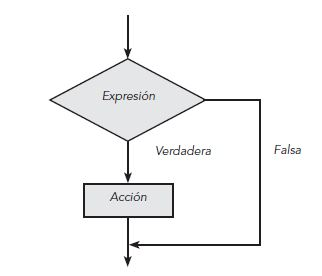
\includegraphics[scale=0.6]{flujoSeleccionSimple}
\end{center}
\end{frame}
%- - - - - - - - - - - - - - - - Slide 05 - - - - - - - - - - - - - - - - - -%
\begin{frame}[t]{Selección sencilla}
\textbf{Ejemplo:} Representar la superación de un examen (Nota >= 5, Aprobado).\\
\vspace{2mm}
\begin{center}
	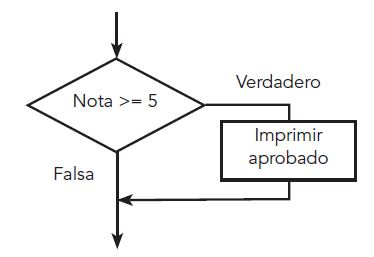
\includegraphics[scale=0.5]{flujoEjemploSeleccionSimple}
\end{center}
\end{frame}

%- - - - - - - - - - - - - - - - Slide 06 - - - - - - - - - - - - - - - - - -%
\begin{frame}[fragile]{Selección sencilla}
\lstinputlisting[style=customc]{codigos/seleccion/ejemploSeleccionSimple.c}
\end{frame}


% *******************************************************************************
% *							SELECCIÓN DOBLE										*
% *******************************************************************************

%- - - - - - - - - - - - - - - - Slide 07 - - - - - - - - - - - - - - - - - -%
\begin{frame}{Selección doble}
En este formato la sentencia \textbf{if} tiene la siguiente sintaxis:\\
\vspace{5mm}
\begin{columns}
	\begin{column}{0.33 \textwidth}
			\begin{block}{\textit{if} (Expresión)}
		Expresión lógica que determina la acción a ejecutar
		\end{block}	
	\end{column}
	\begin{column}{0.33 \textwidth}
		\begin{block}{Accion$ _{1} $}
			Acción que se realiza si la expresión lógica es verdadera.
		\end{block}	
	\end{column}
	\begin{column}{0.33 \textwidth}
		\begin{block}{\textit{else} Accion$ _2 $}
			Acción que se ejecuta si la expresión lógica es falsa.
		\end{block}
	\end{column}
\end{columns}
\end{frame}

%- - - - - - - - - - - - - - - - Slide 08 - - - - - - - - - - - - - - - - - -%
\begin{frame}{Selección doble}
Acción$ _{1} $ y Acción$ _{2} $, son individualmente, o bien una única instrucción que termina en
un punto y coma (;) o un grupo de instrucciones encerradas entre llaves.\\
\vspace{2mm}
Si \textit{Expresión} es verdadera, se ejecuta \textit{Acción$ _{1} $} y en caso contrario se ejecuta \textit{Acción$ _{2} $}
\begin{center}
	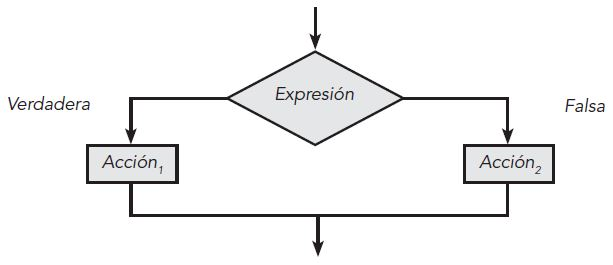
\includegraphics[width=0.7\linewidth]{figs/flujoSeleccionDoble}
\end{center}
\end{frame}

%- - - - - - - - - - - - - - - - Slide 09 - - - - - - - - - - - - - - - - - -%
\begin{frame}[fragile]{Selección doble}
\textbf{Ejemplo:} Calcular el mayor de dos números leídos del teclado y visualizarlo en pantalla.
%\begin{lstlisting}
%#include<stdio.h>
%
%int main(void)
%{
%    int x, y;
%    printf("Ingrese el primer valor: ");
%}
%\end{lstlisting}
\lstinputlisting[style=customc]{codigos/seleccion/ejemploSeleccionDoble.c}
\end{frame}

% *******************************************************************************
% *							SELECCIÓN MULTIPLE									*
% *******************************************************************************
%- - - - - - - - - - - - - - - - Slide 10 - - - - - - - - - - - - - - - - - -%
\begin{frame}[t, fragile]{Selección Multiple}
	Una sentencia \textbf{if} es anidada cuando la sentencia de la rama verdadera o la rama falsa es a su vez una sentencia if. Una sentencia \textbf{if} anidada se puede utilizar para implementar decisiones con varias alternativas o multialternativas.
	\begin{columns}
		\begin{column}{0.40 \textwidth}
		  \centering
			{\LARGE SINTAXIS:}
		\end{column}
		\begin{column}{0.40 \textwidth}
            \vspace{1.5mm}
			\begin{lstlisting}
if(condición_1)
    sentencia_1
else if(condicion_2)
    sentencia_2
    .
    .
else if(condicion_n-1)
    sentencia_n-1
else
    sentencia_n
\end{lstlisting}
		\end{column}	
	\end{columns}
\end{frame}

%- - - - - - - - - - - - - - - - Slide 10 - - - - - - - - - - - - - - - - - -%
\begin{frame}[c]{Selección Multiple}
La sentencia \textbf{switch} es una sentencia que se utiliza para seleccionar una de múltiples alternativas. Es especialmente útil cuando la selección se basa en el valor de una variable simple o de una expresión simple denominada \textbf{\textit{expresión de control}} o \textbf{\textit{selector}}. El valor de esta expresión puede ser de tipo \textit{\textbf{int}} o \textbf{\textit{char}}, pero no de tipo float ni double.
\end{frame}

%- - - - - - - - - - - - - - - - Slide 11 - - - - - - - - - - - - - - - - - -%
\begin{frame}[fragile]{Selección Multiple}
\centering
{\LARGE SINTAXIS}
    \begin{lstlisting}
switch (selector)
{
    case etiqueta1 : sentencias1;
    case etiqueta2 : sentencias2;
    .
    .
    case etiquetan : sentenciasn;
    default: sentencias; /* opcional */
}
\end{lstlisting}
\end{frame}


%- - - - - - - - - - - - - - - - Slide 12 - - - - - - - - - - - - - - - - - -%
\begin{frame}[t]{Selección Multiple}
\hspace{5mm}La expresión de control o \textbf{selector} se evalúa y se compara con cada una de las etiquetas de \textbf{case}. Cada etiqueta es un valor único, constante y cada etiqueta debe tener un valor diferente de los otros.\\
\hspace{5mm}Si el valor de la expresión selector es igual a una de las etiquetas case, por ejemplo, etiqueta1, entonces
la ejecución comenzará con la primera sentencia de la secuencia y continuará hasta que se encuentre el final de la sentencia de control switch, o hasta encontrar la sentencia \textbf{break}.\\
\hspace{5mm}Típicamente después de cada bloque se sitúa la sentencia \textbf{break }como última sentencia del bloque. La sentencia \textbf{break} hace que siga la ejecución en la siguiente sentencia al switch.
\end{frame}

%- - - - - - - - - - - - - - - - Slide 13 - - - - - - - - - - - - - - - - - -%
\begin{frame}[c,fragile]{Selección Multiple}
\centering
SINTAXIS CON break
\begin{lstlisting}
switch (selector)
{
    case etiqueta1 : sentencias1;
    break;
    case etiqueta2 : sentencias2;
    break;
    .
    .
    .
    case etiquetan :sentenciasn;
    break;
    default: sentenciasd; /* opcional */
}
\end{lstlisting}
\end{frame}

%- - - - - - - - - - - - - - - - Slide 14 - - - - - - - - - - - - - - - - - -%
\begin{frame}[c,fragile]{Selección Multiple}
\centering
Elección de tres opciones y un valor en forma predeterminada.
\begin{lstlisting}
switch (opcion)
{
    case 0:
        printf("Cero!");
        break;
    case 1:
        printf("Uno!");
        break;
    case 2:
        printf("Dos!");
        break;
    default:
        printf("Fuera de rango");
}
\end{lstlisting}
\end{frame}


%- - - - - - - - - - - - - - - - Slide 15 - - - - - - - - - - - - - - - - - -%
\begin{frame}[c,fragile]{Selección Multiple}
\centering
Selección múltiple, tres etiquetas ejecutan la misma sentencia.
\begin{lstlisting}
switch (opcion)
{
    case 0:
    case 1:
    case 2:
        printf("Menor de 3");
        break;
    case 3:
        printf("Igual a 3");
        break;
    default:
        printf("Mayor que 3");
}
\end{lstlisting}
\end{frame}


%- - - - - - - - - - - - - - - - Slide 16 - - - - - - - - - - - - - - - - - -%
\begin{frame}[fragile]{Selección Multiple}
Comparación de las sentencias if-else-if y switch. Se necesita saber si un determinado
carácter car es una vocal. Solución con if-else-if.
\vspace{2mm}
    \begin{columns}
        \begin{column}{0.4 \textwidth}
            \begin{lstlisting}[basicstyle=\ttfamily\tiny]
if((car=='a')||(car=='A'))
   printf("%c es una vocal\n",car);
else if((car=='e')||(car=='E'))
   printf("%c es vocal\n",car);
else if((car=='i')||(car=='I'))
   printf("%c es vocal\n",car);
else if((car=='o')||(car=='O'))
   printf("%c es vocal\n",car);
else if((car=='u')||(car=='U'))
   printf("%c es vocal\n",car);
else
   printf("%c no es vocal\n",car);
\end{lstlisting}
        \end{column}
        \begin{column}{0.5 \textwidth}
            \begin{lstlisting}[basicstyle=\ttfamily\tiny]
switch (car)
{
    case 'a': case 'A':
    case 'e': case 'E':
    case 'i': case 'I':
    case 'o': case 'O':
    case 'u': case 'U':
        printf("%c es una vocal\n",car);
        break;
    default:
       printf("%c no es una vocal\n",car);
}
\end{lstlisting}
        \end{column}
    \end{columns}

\end{frame}


%\begin{frame}[c]{Selección sencilla}
%La estructura selectiva \textbf{SI - ENTONCES} permite que el flujo de datos siga por un camino específico si se cumple una condición o conjunto de condiciones. \\
%\vspace*{2mm}
%Si al evaluar la condición (o condiciones) el resultado es verdadero, entonces se ejecutan un conjunto de operaciones. \\
%\vspace*{2mm}
%Luego, se continúa con la secuencia normal del flujo.\\
%\vspace{28mm}
%\tiny Battistutti, O. C. (2005). Metodología de la programación: Algoritmos, diagramas de flujo y programas (3rd ed.). México, D.F.: Alfaomega.
%\end{frame}


%- - - - - - - - - - - - - - - - Slide 04 - - - - - - - - - - - - - - - - - -%
%\begin{frame}[c]{Diagrama de flujo de la selección sencilla}
%\vspace*{4mm}
%\begin{center}
%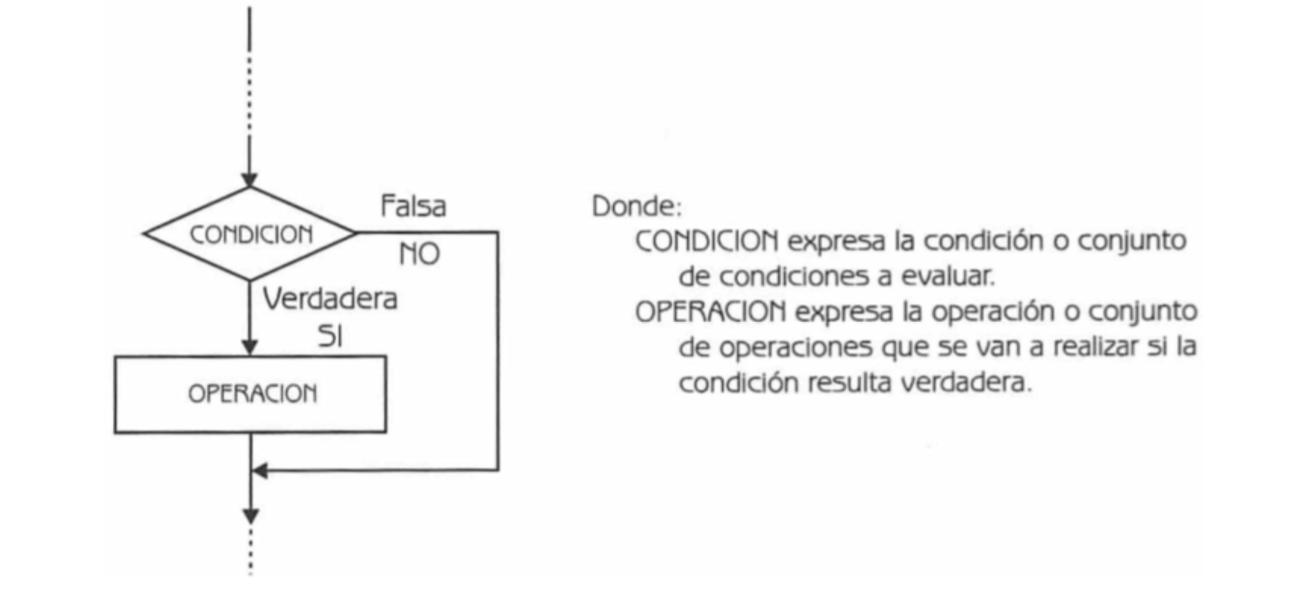
\includegraphics[scale=0.45]{figs/SeleccionSencillaDF.png}
%\end{center}
%\vspace*{-6mm}
%\tiny Battistutti, O. C. (2005). Metodología de la programación: Algoritmos, diagramas de flujo y programas (3rd ed.). México, D.F.: Alfaomega.
%\end{frame}


%- - - - - - - - - - - - - - - - Slide 05 - - - - - - - - - - - - - - - - - -%
%\begin{frame}[fragile, c] \frametitle{Estructura de la selección sencilla}
%\begin{lstlisting}
%...
%if(CONDICION)
%{
%    OPERACION
%}
%...
%\end{lstlisting}
%\vspace*{35mm}
%%\tiny Aguilar, L. J., & Martínez, I. Z. (2010). Programación en C: Metodología, algoritmos y estructura de datos. Madrid: McGraw-Hill.
%\end{frame}


%- - - - - - - - - - - - - - - - Slide 06 - - - - - - - - - - - - - - - - - -%



%- - - - - - - - - - - - - - - - Slide 07 - - - - - - - - - - - - - - - - - -%



%- - - - - - - - - - - - - - - - Slide 08 - - - - - - - - - - - - - - - - - -%



%- - - - - - - - - - - - - - - - Slide 09 - - - - - - - - - - - - - - - - - -%

    \section{Teoría de Ciclos}

% - - - - - - - - - - - - - - - - - - - - - Slide 01 - - - - - - - - - - - - - - - - - - - - - - -
\begin{frame}{Teoría de Ciclos}
    \begin{center}\textbf{Definición}\end{center}
    \justify
    \hspace{5mm}
    Un bucle (ciclo o lazo, loop en inglés) es cualquier construcción de programa que
    repite una sentencia o secuencia de sentencias un número de veces. La sentencia (o
    grupo de sentencias) que se repiten en un bloque se denomina cuerpo del bucle y
    cada repetición del cuerpo del bucle se llama iteración del bucle.
\end{frame}


% - - - - - - - - - - - - - - - - - - - - - Slide 02 - - - - - - - - - - - - - - - - - - - - - - -
\begin{frame}{Teoría de Ciclos}
    \begin{center}\textbf{Contadores}\end{center}
    \vspace{-2mm}
    Es una variable cuyo valor se incrementa o decrementa en una cantidad constante cada vez que se produce un determinado suceso o acción en cada repetición; dicha variable controla o determina la cantidad de veces que se repite un proceso o dato.
    \begin{block}{Contadores}
        int contador 5 1; //variable con valor inicial de 1\\
        contador++; o ++contador; o contador+=1;
    \end{block}
\end{frame}


% - - - - - - - - - - - - - - - - - - - - - Slide 03 - - - - - - - - - - - - - - - - - - - - - - -
\begin{frame}{Teoría de Ciclos}
    \vspace{-1mm}
    \begin{center}\textbf{Acumuladores}\end{center}
    \vspace{-3mm}
    Un acumulador realiza la misma función que un contador con la diferencia de que el incremento o decremento es variable. Es una variable que acumula sobre sí misma un conjunto de valores, para tener la acumulación de todos ellos en una sola variable. Almacena cantidades resultantes de operaciones sucesivas.
    \begin{block}{Acumuladores}
        int acumulador 50;\\
        acumulador = acumulador + valor;
    \end{block}
\end{frame}


% - - - - - - - - - - - - - - - - - - - - - Slide 04 - - - - - - - - - - - - - - - - - - - - - - -
\begin{frame}{Teoría de Ciclos}
    \begin{center}\textbf{Centinela}\end{center}
    \hspace{5mm}
    El centinela es una variable que inicia con un valor, luego dentro de un bucle este valor cambia, haciendo falsa la condición del ciclo y por lo tanto indicará el fin del ciclo (el usuario puede determinar cuándo hacerlo). La repetición controlada por centinela se considera como una repetición indefinida (se desconoce el número de repeticiones).
\end{frame}



% - - - - - - - - - - - - - - - - - - - - - Slide 05 - - - - - - - - - - - - - - - - - - - - - - -
\begin{frame}{Teoría de ciclos}

    \begin{center}\textbf{Ciclo While}\end{center}
    \hspace{5mm}
    Un ciclo \textbf{while} tiene una condición (expresión lógica) que controla la secuencia de repetición. La posición de esta condición es previo al cuerpo del ciclo, de modo que, cuando se ejecuta, se evalúa la condición antes de que se ejecute el cuerpo del bucle.
\end{frame}


% - - - - - - - - - - - - - - - - - - - - - Slide 06 - - - - - - - - - - - - - - - - - - - - - - -
\begin{frame}[fragile]{Tipos de Ciclos}
\begin{center}\textbf{Sintaxis}\end{center}
\begin{columns}[t]
    \begin{column}{0.4 \textwidth}
        \begin{lstlisting}
while(condicion)
    sentencia;
\end{lstlisting}
    \end{column}
    \begin{column}{0.4 \textwidth}
        \begin{lstlisting}
while(condicion)
{
    senctencia_1;
    .
    .
    sentencia_n;
}
\end{lstlisting}
    \end{column}
\end{columns}
\end{frame}


% - - - - - - - - - - - - - - - - - - - - - Slide 07 - - - - - - - - - - - - - - - - - - - - - - -
\begin{frame}[t]{Teoría de ciclos}
    \vspace{-5mm}
    \begin{center}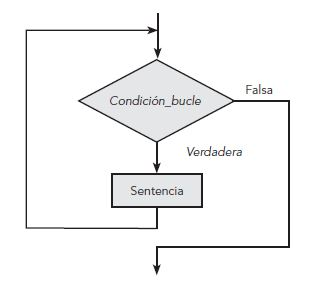
\includegraphics[scale=0.4]{flujoWhile.JPG}\vspace{-5mm}\end{center}
    \justify
    \hspace{5mm}
    El diagrama indica que la ejecución de la sentencia se repite mientras la condición permanece verdadera y termina cuando se hace falsa. También que la condición del ciclo se evalúa antes de ejecutar el cuerpo del ciclo, si esta condición es inicialmente falsa, el cuerpo del ciclo no se ejecutará. En otras palabras, el cuerpo de un bucle while se ejecutará cero o más veces.
\end{frame}



% - - - - - - - - - - - - - - - - - - - - - Slide 08 - - - - - - - - - - - - - - - - - - - - - - -
\begin{frame}[fragile]{Teoría de ciclos}
\begin{center}
    \textbf{CICLO DE MUESTRA CON \textit{WHILE}}
\end{center}
\lstinputlisting[style=customc]{codigos/ciclos/cicloMuestra.c}
\end{frame}



% - - - - - - - - - - - - - - - - - - - - - Slide 09 - - - - - - - - - - - - - - - - - - - - - - -
\begin{frame}[fragile]{Teoría de ciclos}
    \begin{center}
        \textbf{Ciclo Infinito}
    \end{center}
    \justify
    Si la variable de control no se actualiza el ciclo se ejecutará “siempre” (ciclo infinito). Un ciclo infinito (sin terminación) se produce cuando la condición del permanece y no se hace falsa en ninguna iteración.
    \vspace{-2mm}
\begin{center}
    \begin{tabular}{c}
            \begin{lstlisting}
/* bucle infinito */
contador = 1;
while (contador < 100)
{
    printf("%d \n", contador);
    contador--;
}
\end{lstlisting}
    \end{tabular}
\end{center}
\end{frame}


% ***********************************************************************************************
% *                                     TIPOS DE CICLOS                                         *
% ***********************************************************************************************
% - - - - - - - - - - - - - - - - - - - - - Slide 10 - - - - - - - - - - - - - - - - - - - - - - -
\begin{frame}{Tipos de ciclos}
\begin{center}
    \textbf{Ciclos controlados por contador}
\end{center}
\justify
\hspace{5mm}
La repectición controlada por un contador se utiliza cuando se conoce el número de repeticiones antes de que un ciclo empiece a ejecutarse; es decir, cuando hay una repetición definida.
\end{frame}

% - - - - - - - - - - - - - - - - - - - - - Slide 11 - - - - - - - - - - - - - - - - - - - - - - -
\begin{frame}{Tipos de ciclos}
\begin{center}
    \textbf{Ciclos controlados por centinela}
    \justify
    \hspace{5mm}
    La repetición controlada por un centinela se utiliza cuando no se conoce el número de repeticiones antes de que un ciclo empiece a ejecutarse; es decir, cuando hay una repetición indefinida.
\end{center}
\end{frame}


% - - - - - - - - - - - - - - - - - - - - - Slide 12 - - - - - - - - - - - - - - - - - - - - - - -
\begin{frame}[fragile,t]{Tipos de ciclos}
    \begin{center}\textbf{Ejemplos}\end{center}
    \begin{columns}[t]
        \begin{column}{0.57 \textwidth}
            \begin{block}{Por contador}
                El siguiente ciclo cuenta hasta 10
                \begin{lstlisting}
int x = 0;
while( x < 10 )
    printf("X: %d\n", x++);
\end{lstlisting}
            \end{block}
        \end{column}
        \begin{column}{0.5 \textwidth}
            \begin{block}{Por centinela}
                Visualizar n asteriscos
                \begin{lstlisting}
contador = 0;
while( contador < n )
{
    printf(" * ");
    contador++;
}/*Fin del while*/
\end{lstlisting}
            \end{block}
        \end{column}
    \end{columns}
\end{frame}

%***************************************************************************
%*                               CICLO FOR                                 *
%***************************************************************************

% - - - - - - - - - - - - - - - - - - - - - Slide 13 - - - - - - - - - - - - - - - - - - - - - - -
\begin{frame}{Tipos de ciclos}{Ciclo For}
\begin{center}
    \textbf{Ciclo For}
\end{center}
La sentencia \textbf{for} es un método para ejecutar un bloque de sentencias un número fijo de veces. El \textit{ciclo \textbf{for}} se diferencia del \textit{ciclo \textbf{while}} en que las operaciones de control del ciclo se sitúan en un solo sitio: la cabecera de la sentencia.
\end{frame}

% - - - - - - - - - - - - - - - - - - - - - Slide 14 - - - - - - - - - - - - - - - - - - - - - - -
\begin{frame}[fragile, t]{Tipos de ciclos}
    \begin{center}
        \textbf{Sintaxis}
    \end{center}
    \vspace{-5mm}
    \begin{lstlisting}[basicstyle=\ttfamily\small]
for(Inicialización; CondiciónIteración;Incremento)
    sentencias
\end{lstlisting}
    \vspace{-3mm}
{\small \begin{description}
    \item[Inicialización:] Inicializa la variable de control del ciclo.\pause
    \item[CondicióIteración:] Expesión lógica que determina se las sentencias se han de ejecutar (mientras sea verdadera)\pause
    \item[Incremento:] Incrementa o decrementa la variable de control de bucle.\pause
    \item[sentencias:] Sentencias a ejecutar en cada iteración del bucle
\end{description}}
\end{frame}


% - - - - - - - - - - - - - - - - - - - - - Slide 15 - - - - - - - - - - - - - - - - - - - - - - -
\begin{frame}{Tipos de ciclos}
    \centering
    \textbf{Diagrama de Flujo del ciclo \textit{For}}\\
    \vspace{3mm}
    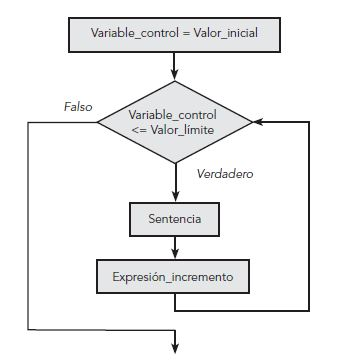
\includegraphics[scale=0.6]{flujoFor.jpg}
\end{frame}



% - - - - - - - - - - - - - - - - - - - - - Slide 16 - - - - - - - - - - - - - - - - - - - - - - -
\begin{frame}[fragile]{Tipos de ciclos}
    \centering
    \textbf{Ejemplo}
    \lstinputlisting[style=customc]{codigos/ciclos/cicloFor.c}
\end{frame}

\begin{frame}{Tipos de ciclos}
    \begin{center}\textbf{Ciclo do-while}\end{center}
    \justify
    La sentencia \textbf{\textit{do-while}} se utiliza para especificar un bucle condicional que se ejecuta al menos una vez. Esta situación se suele dar en algunas circunstancias en las que se ha de tener la seguridad de que una determinada acción se ejecutará una o varias veces, pero al menos una vez.
\end{frame}

% - - - - - - - - - - - - - - - - - - - - - Slide 17 - - - - - - - - - - - - - - - - - - - - - - -
\begin{frame}[fragile]{Tipos de ciclos}
    \begin{center}\textbf{SIntaxis}\end{center}
    \begin{columns}
        \begin{column}{0.5 \textwidth}
            \begin{lstlisting}
do
    sentencia
while(expresion);
            \end{lstlisting}
        \end{column}
        \begin{column}{0.5 \textwidth}
            \begin{lstlisting}
do
{
    sentencias;
}while(expresion);
            \end{lstlisting}
        \end{column}
    \end{columns}
\end{frame}

% - - - - - - - - - - - - - - - - - - - - - Slide 17 - - - - - - - - - - - - - - - - - - - - - - -
\begin{frame}{Tipos de ciclos}
    \begin{center}\textbf{Sintaxis}\end{center}
    \begin{columns}
        \begin{column}{0.5 \textwidth}
                \hspace{2mm}
                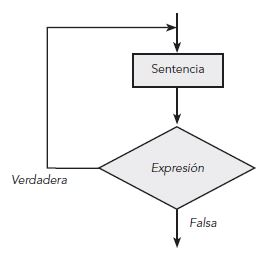
\includegraphics[scale=0.7]{flujoDoWhile.jpg}
        \end{column}
        \begin{column}{0.5 \textwidth}
            \justify
            Después de cada ejecución de sentencia se evalúa expresión: si es falsa, se termina el
            ciclo y se ejecuta la siguiente sentencia; si es verdadera, se repite el cuerpo del ciclo (la sentencia).
        \end{column}
    \end{columns}
\end{frame}

\begin{frame}[fragile]{Tipos de ciclos}
    \begin{center}\textbf{Ejemplo}\end{center}
    \lstinputlisting[style=customc]{codigos/ciclos/cicloDoWhile.c}
\end{frame}
    \section*{Cadenas de Caracteres}

%- - - - - - - - - - - - - - - - - Título - - - - - - - - - - - - - - - - - -%
\begin{frame}[c] 
\centering
\huge \textbf{Cadenas de caracteres}
\end{frame}

%- - - - - - - - - - - - - - - - - - - - - Slide 01 - - - - - - - - - - - - - - - - - - - - -
\begin{frame}[t, fragile]
    \frametitle{Cadena de caracteres}
    \justify
    \hspace{5mm}En el lenguaje C no existe el tipo de dato cadena (string) como en otros lenguajes de programación, por lo que se utiliza un arreglo (lista finita de n cantidad de elementos del mismo tipo) de caracteres, para poder almacenar una cadena:
    \begin{lstlisting}
                char cad[] = "Lenguaje";
\end{lstlisting}
    \vspace{-2mm}
    \hspace{5mm}Una cadena de caracteres es un arreglo de caracteres que contiene al final el carácter nulo ( $\backslash$0); por esta razón es necesario que al declarar los arreglos éstos sean de un carácter más que la cadena más grande. El compilador inserta automáticamente un carácter nulo al final de la cadena, de modo que la secuencia real sería:
    \begin{lstlisting}
                char cad[9] = "Lenguaje";
\end{lstlisting}
\end{frame}


%- - - - - - - - - - - - - - - - - - - - - Slide 02 - - - - - - - - - - - - - - - - - - - - -
\begin{frame}
    \frametitle{Cadena de caracteres}
    \begin{center}\textbf{Lectura}\end{center}
    \justify
    \hspace{5mm}Una opción para almacenar una cadena de caracteres es el uso de la palabra reservada \textbf{scanf(variable)} pero, si queremos almacenar una cadena con espacios en blanco no lo podemos hacer con ella, sino que debemos utilizar la palabra reservada \textbf{gets}, que se encuentra dentro de la librería string.h; \textbf{gets} sólo se utiliza para leer cadenas de caracteres y scanf para leer cualquier tipo de variable, de preferencia de tipo numérico.
\end{frame}

%- - - - - - - - - - - - - - - - - - - - - Slide 03 - - - - - - - - - - - - - - - - - - - - -
\begin{frame}
    \frametitle{Cadena de caracteres}
    \centering
    Ejemplo:
    \lstinputlisting[style=customc]{codigos/cadenas/ejemploLecturaEscritura.c}
\end{frame}



%- - - - - - - - - - - - - - - - - - - - - Slide 04 - - - - - - - - - - - - - - - - - - - - -
\begin{frame}
    \frametitle{Cadena de caracteres}
    \begin{center}\textbf{Escritura}\end{center}
    La función \textbf{puts()}, escribe una cadena de caracteres de salida y remplaza el caracter nulo de terminación de la cadena ($\backslash$0) por el carácter de nueva línea ($\backslash$n).
\end{frame}



%- - - - - - - - - - - - - - - - - - - - - Slide 05 - - - - - - - - - - - - - - - - - - - - -
\begin{frame}[fragile]
    \frametitle{Cadena de caracteres}
    \begin{center}\textbf{Asignación de Cadenas}\end{center}
    \justify
    \hspace{5mm}C soporta dos métodos para asignar cadenas. Uno de ellos, ya visto anteriormente, cuando se inicializaban las variables de cadena. La sintaxis utilizada:
    \begin{lstlisting}
char cadena[longitudCadena] = "ConstanteCadena";
    \end{lstlisting}
\end{frame}


%- - - - - - - - - - - - - - - - - - - - - Slide 06 - - - - - - - - - - - - - - - - - - - - -
\begin{frame}[fragile]
    \frametitle{Cadena de caracteres}
    \begin{center}\textbf{Asignación de Cadenas}\end{center}
    \hspace{5mm}El segundo método para asignación de una cadena a otra es utilizar la función strcpy( ). La función copia los caracteres de la cadena fuente a la cadena destino. La cadena destino debe tener espacio suficiente para contener toda la cadena fuente. El prototipo de la función:
    \begin{lstlisting}
    char* strcpy(char* destino, const char* fuente);
    \end{lstlisting}
    Una vez definido el arreglo de caracteres, se le asigna una cadena constante:
    \begin{lstlisting}
char nombre[41];
strcpy(nombre, "Cadena a copiar");\end{lstlisting}
\end{frame}


%- - - - - - - - - - - - - - - - - - - - - Slide 07 - - - - - - - - - - - - - - - - - - - - -
\begin{frame}[fragile]
    \frametitle{Cadena de caracteres}
    \begin{center}\textbf{Comparación de Cadenas}\end{center}
    La biblioteca string.h proporciona un conjunto de funciones que comparan cadenas. Estas funciones comparan los caracteres de dos cadenas utilizando el valor ASCII de cada carácter. La funcion es strcmp( ).
    \begin{lstlisting}
    int strcmp(const char* cad1, const char* cad2);
    \end{lstlisting}
    La función compara las cadenas cad1 y cad2. El resultado entero es:
    \begin{itemize}
        \item $ < $ 0 si cad1 es menor que cad2.
        \item $ = $ 0 si cad1 es igual a cad2.
        \item $ > $ 0 si cad1 es mayor que cad2.
    \end{itemize}
\end{frame}



%- - - - - - - - - - - - - - - - - - - - - Slide 08 - - - - - - - - - - - - - - - - - - - - -
\begin{frame}[fragile]
    \frametitle{Cadena de caracteres}
    \begin{center}\textbf{Ejemplo de Comparación de Cadenas}\end{center}
    \begin{lstlisting}[basicstyle=\ttfamily\tiny]
    char cad1[ ] = "Microsoft C";
    char cad2[ ] = "Microsoft Visual C"
    int i;
    i = strcmp(cad1, cad2); /*i, toma un valor negativo */
    strcmp("Waterloo", "Windows") /*< 0 {Devuelve un valor negativo}*/
    strcmp("Mortimer", "Mortim") /*> 0 {Devuelve un valor positivo}*/
    strcmp("Jertru", "Jertru") /*= 0 {Devuelve cero}*/
    \end{lstlisting}
\end{frame}
    \section*{Arreglos unidimencionales}
% - - - - - - - - - - - - - - - - - - - - Slide01 - - - - - - - - - - - - - - - - -
\begin{frame}
    \frametitle{Arreglos Unidimencionales}
    \framesubtitle{Definición e Inicialización}
    \begin{center}
        \textbf{Definición}
    \end{center}
    \justify
    \hspace{5mm}Un arreglo es un tipo de dato estructurado que almacena en una sola variable un conjunto limitado de elementos del mismo tipo. El nombre del arreglo apunta a la dirección del primer elemento del arreglo. Los datos se llaman elementos del arreglo y su posición se numera consecutivamente: 1, 2, 3…n. Un arreglo inicia en la posición cero, por lo tanto el i-ésimo elemento está en la posición i-1, es decir si el arreglo llamado \textbf{a} tiene \textbf{\textit{n}} elementos, sus nombres son a[0], a[1], ..., a[n-1].\\
\end{frame}


% - - - - - - - - - - - - - - - - - - - - Slide02 - - - - - - - - - - - - - - - - -
\begin{frame}
\frametitle{Arreglos Unidimencionales}
\framesubtitle{Definición e Inicialización}
    \justify
    Para acceder a un elemento específico de un arreglo se usa un índice o subíndice.
    Un arreglo se caracteriza por:
    \begin{enumerate}
        \item Ser una lista de un número finito de n elementos del mismo tipo.
        \item Almacenar los elementos del arreglo en memoria contigua.
        \item Tener un único nombre de variable que representa a todos los elementos y éstos se diferencian por un índice o subíndice.
        \item Acceder de manera directa o aleatoria a los elementos individuales del arreglo, por el nombre del arreglo y el índice o subíndice.
    \end{enumerate}
\end{frame}


% - - - - - - - - - - - - - - - - - - - - Slide03 - - - - - - - - - - - - - - - - -
\begin{frame}[fragile]
    \frametitle{Arreglos Unidimencionales}
    \framesubtitle{Definición e Inicialización}
    Formato para declarar un arreglo unidimencional.
    \vspace{2mm}
    \begin{lstlisting}
        tipoDato identifArreglo[tamArreglo];
\end{lstlisting}
Donde:
\begin{itemize}
    \item \textbf{tipoDato} se refiere al tipo de dato de cada elemento del arreglo; puede ser entero, real, carácter, etcétera.
    \item \textbf{identifArreglo} es el nombre que representa a todo el arreglo
    \item \textbf{tamArreglo} es la cantidad de elementos que contiene el arreglo.
\end{itemize}
\end{frame}


% - - - - - - - - - - - - - - - - - - - - Slide04 - - - - - - - - - - - - - - - - -
\begin{frame}[fragile, t]
    \frametitle{Arreglos Unidimencionales}
    \framesubtitle{Definición e Inicialización}
    \begin{center}\textbf{Ejemplo}\end{center}
        \vspace{-4mm}
    \begin{lstlisting}
float x[8];
    \end{lstlisting}
    \vspace{-5mm}
\begin{center}
        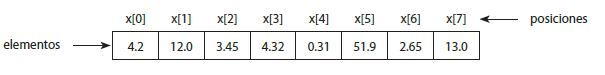
\includegraphics[scale=0.55]{figs/ejemploArregloUnidimencional}
\end{center}
\vspace{-6mm}
\justify
\hspace{5mm}Este arreglo contiene ocho elementos almacenados entre la posición (0-7). Para referirnos a un elemento en particular dentro del arreglo, especificamos el nombre del arreglo y el número de posición donde se encuentra ubicado. La posición del arreglo va entre corchetes (“[ ]”).
\end{frame}


% - - - - - - - - - - - - - - - - - - - - Slide05 - - - - - - - - - - - - - - - - -
\begin{frame}[fragile]
    \frametitle{Arreglos Unidimencionales}
    \framesubtitle{Definición e Inicialización}
    Si la instrucción fuera imprimir \textbf{x[4]} se mostrará el valor de 0.31\\
    \begin{lstlisting}
printf("%f", x[4]);
    \end{lstlisting}
    Para almacenar la suma de los valores contenidos en los primeros tres elementos del arreglo x, escribiríamos:\\
    \begin{lstlisting}
a = x[0] + x[1] + x[2];
printf("%f", a);
    \end{lstlisting}
    Para dividir el valor del séptimo elemento del arreglo x entre 2 y asignar el resultado a la variable c escribiríamos:
    \begin{lstlisting}
c = x[6]/2;
    \end{lstlisting}
\end{frame}

% - - - - - - - - - - - - - - - - - - - - Slide06 - - - - - - - - - - - - - - - - -
\begin{frame}[fragile,t]
    \frametitle{Arreglos Unidimencionales}
    \framesubtitle{Definición e Inicialización}
    \begin{center}
        \textbf{Inicialización}
    \end{center}
    En el momento de declarar el arreglo, se especifican los valores.
    \begin{lstlisting}
/*tipoDato identif[tamArreglo]={valores};*/
int lista[5] = {10,17,8,4,9};
    \end{lstlisting}
    \vspace{-3mm}
    Para llenar un arreglo completo se utiliza generalmente el ciclo desde \textbf{(for}) facilitando con la variable de control el incremento de la \textbf{\textit{i}}, donde la \textbf{\textit{i}} representa el subíndice.
    \begin{lstlisting}
for(i=0;i<5;i++)
    printf("%d", lista[i]);
    \end{lstlisting}
\end{frame}


% - - - - - - - - - - - - - - - - - - - - Slide07 - - - - - - - - - - - - - - - - -
\begin{frame}[fragile]
    \frametitle{Arreglos Unidimencionales}
    \framesubtitle{Definición e Inicialización}
    \begin{center}
        \textbf{Modificación}
    \end{center}
    \justify
    Para modificar los elementos de un vector en cualquier momento, sólo es necesario especificar el nombre del arreglo unidimensional, la posición y el nuevo valor. Enseguida se muestra la sintaxis a seguir:
    \begin{lstlisting}
/*tipoDato identArr[pos]=valor;*/
int b[3] = 18;
    \end{lstlisting}
    Donde \textbf{valor} es un dato, el resultado de alguna operación lógica o aritmética, etc.
\end{frame}
    \section*{Arreglos Bidimencionales}

% - - - - - - - - - - - - - - - - - Slide 01 - - - - - - - - - - - - - - - -
\begin{frame}
\frametitle{Arreglos Bidimencionales}
\end{frame}


% - - - - - - - - - - - - - - - - - Slide 02 - - - - - - - - - - - - - - - -
\begin{frame}
\frametitle{Arreglos Bidimencionales}
\end{frame}

% - - - - - - - - - - - - - - - - - Slide 03 - - - - - - - - - - - - - - - -
\begin{frame}
\frametitle{Arreglos Bidimencionales}
\end{frame}

% - - - - - - - - - - - - - - - - - Slide 04 - - - - - - - - - - - - - - - -
\begin{frame}
\frametitle{Arreglos Bidimencionales}
\end{frame}

% - - - - - - - - - - - - - - - - - Slide 05 - - - - - - - - - - - - - - - -
\begin{frame}
\frametitle{Arreglos Bidimencionales}
\end{frame}

% - - - - - - - - - - - - - - - - - Slide 06 - - - - - - - - - - - - - - - -
\begin{frame}
\frametitle{Arreglos Bidimencionales}
\end{frame}
    \section*{Definición de Función}

%- - - - - - - - - - - - - - - - - Título - - - - - - - - - - - - - - - - - -%
\begin{frame}[c] 
\centering
\huge \textbf{Definición de Funcion}
\end{frame}



% - - - - - - - - - - - - - - - - - Slide 01 - - - - - - - - - - - - - - - -
\begin{frame}
    \frametitle{Definición de Funcion}
    \justify
    \hspace{5mm}Un problema difícil es más sencillo al dividirlo en pequeñas partes y tratar de buscar la solución de cada una de ellas y así resolver todo el problema general, la mejor forma de elaborar
    y dar mantenimiento a un programa complejo es construirlo a partir de bloques menores o módulos.\\
    \hspace{5mm}Dichos módulos se escriben solamente una vez, pero pueden ser llamados en diferentes puntos del programa principal o de cualquier otro módulo.
\end{frame}


% - - - - - - - - - - - - - - - - - Slide 02 - - - - - - - - - - - - - - - -
\begin{frame}
\frametitle{Definición de Funcion}
\justify
\hspace{5mm}En lenguaje C a cada módulo o subprograma se le conoce como función; en este lenguaje se trabaja a base de funciones y, de manera general, los programas se elaboran combinando funciones que el programador escribe y funciones “predefinidas” disponibles en la biblioteca estándar de C.
\begin{center}
    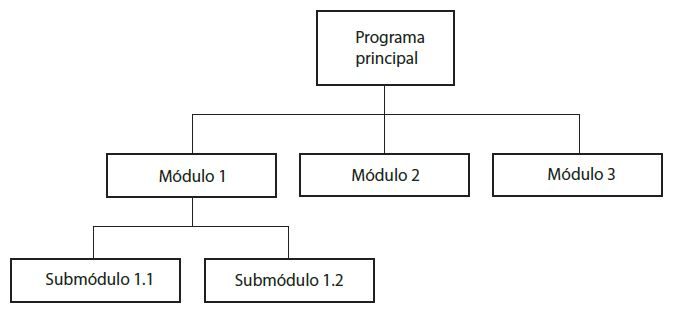
\includegraphics[scale=0.4]{figs/diagramaProgramacionModular.jpg}
\end{center}
\end{frame}



% - - - - - - - - - - - - - - - - - Slide 03 - - - - - - - - - - - - - - - -
\begin{frame}
    \frametitle{Definición de Funcion}
    \begin{center}
        \textbf{Ventajas de la programación modular}
    \end{center}
    \vspace{-8mm}
    \begin{itemize}
        \item Facilita el diseño descendente \textit{(proceso mediante el cual un problema se descompone en un serie de niveles o pasos sucesivos)}.\pause
        \item Se simplifica un algoritmo complejo.\pause
        \item Cada módulo se puede elaborar de manera independiente, lo que permite trabajar simultáneamente a varios programadores y disminuir el tiempo de elaboración del algoritmo.\pause
        \item La depuración se lleva a cabo en cada módulo.\pause
        \item El mantenimiento es más sencillo.\pause
        \item Creación de bibliotecas con módulos específicos (se pueden utilizar en otros programas).
    \end{itemize}
\end{frame}



% - - - - - - - - - - - - - - - - - Slide 04 - - - - - - - - - - - - - - - -
\begin{frame}
\frametitle{Definición de Funcion}
\begin{center}
    \textbf{Función}
\end{center}
\hspace{5mm}Es un subprograma que realiza una tarea específica que puede o no recibir valores (parámetros). En C podemos devolver cualquier tipo de datos escalares tipo numérico y el tipo carácter o en su caso regresar un valor nulo que llamaremos nada o ninguno). El uso de funciones es una práctica común y recomendable ya que permite dividir el código, simplificando así el desarrollo y la depuración del mismo.
\end{frame}
    \section*{Prototipos, llamada y cuerpo de la función}

%- - - - - - - - - - - - - - - - - Título - - - - - - - - - - - - - - - - - -%
\begin{frame}[c] 
\centering
\huge \textbf{Prototipos, llamada y cuerpo de la función}
\end{frame}



% - - - - - - - - - - - - - - - - - Slide 01 - - - - - - - - - - - - - - - -
\begin{frame}[t]
    \frametitle{Prototipos, llamada y cuerpo de la función}
    \begin{center}
        \textbf{Prototipo}
    \end{center}
    \vspace{-6mm}
    \hspace{5mm}Un prototipo es el encabezado de una función, es decir la primera línea de la función. La ventaja de utilizar prototipos es que las funciones pueden estar en cualquier lugar y en cualquier orden y pueden ser llamadas desde cualquier punto del programa principal o de otra función.
    \vspace{-2mm}
    \begin{block}{Orden}
        \begin{enumerate}
            \item Declaración de los prototipos de cada función.\pause
            \item Cuerpo de la función principal.\pause
            \item Al final el cuerpo de cada función.
        \end{enumerate}
    \end{block}
\end{frame}



% - - - - - - - - - - - - - - - - - Slide 02 - - - - - - - - - - - - - - - -
\begin{frame}[fragile]
    \frametitle{Prototipos, llamada y cuerpo de la función}
    \begin{center}
        \textbf{EJEMPLO}
    \end{center}
    \begin{lstlisting}[basicstyle=\ttfamily\tiny]
#librearias
#Constantes
funcionA();/*Prototípo de la función A*/
funcionB();/*Prototípo de la función B*/
int main(){
    variables
    Cuerpo del programa principal
    ............
    funcionaA();
    funcionaB();
    .......
    return 0;
}
funcionA(){
    variables locales de función
    instrucciones
}
funcionB(){
    variables locales de función
    instrucciones
}
\end{lstlisting}
\end{frame}

    \section*{Funciones Sencillas}

%- - - - - - - - - - - - - - - - - Título - - - - - - - - - - - - - - - - - -%
\begin{frame}[c] 
\centering
\huge \textbf{Funciones Sencillas}
\end{frame}



% - - - - - - - - - - - - - - - - - Slide 01 - - - - - - - - - - - - - - - -
\begin{frame}[fragile]{Funciones Sencillas}
\hspace{5mm}Son aquellas que no reciben parámetros o valores, ya que éstos se solicitan dentro de la función, luego se realizan las instrucciones (cálculos u operaciones) y normalmente se imprime el resultado.\\Ejemplo:
\begin{lstlisting}
void nombreFuncion() {
    Declaracion de variables;
    Cuerpo de la funcion;
    .
    .
}
\end{lstlisting}
\end{frame}



% - - - - - - - - - - - - - - - - - Slide 01 - - - - - - - - - - - - - - - -
\begin{frame}[fragile]{Funciones Sencillas}
\begin{center}
    \textbf{Llamadas a funciones sin paso de parametros}
\end{center}
\begin{lstlisting}
    printf("%d", nombreFuncion());
    
    variable = nombreFuncion();
    
    if(nombreFuncion() > expresion)
\end{lstlisting}
\end{frame}
    \section*{Funciones con parámetro por valor y que regresan valor}

%- - - - - - - - - - - - - - - - - Título - - - - - - - - - - - - - - - - - -%
\begin{frame}[c] 
\centering
\huge \textbf{Funciones con parámetros por valor y\\que regresan valor}
\end{frame}



%- - - - - - - - - - - - - - - - - Slide 01 - - - - - - - - - - - - - - - - - -%
\begin{frame}
    \frametitle{Funciones con parámetros por valor y que regresan valor}
    Estas funciones son las más utilizadas en la programación ya que pueden recibir uno o más valores llamados
    parámetros y regresan un solo valor de tipo entero, real o carácter. Si deseas regresar un arreglo de carácter
    es necesario hacerlo desde los parámetros. Los parámetros o valores son enviados del programa principal
    o de otra función. Dentro de la función se realizan solamente las instrucciones (cálculos u operaciones). Es
    importante revisar que el tipo de dato que regresará la función sea del mismo tipo que el valor declarado en
    el encabezado de la misma.
\end{frame}



%- - - - - - - - - - - - - - - - - Slide 02 - - - - - - - - - - - - - - - - - -%
\begin{frame}
\frametitle{Funciones con parámetros por valor y que regresan valor}
\begin{center}
    \textbf{Parámetros de una Función}
\end{center}
También son llamados argumentos y se corresponden con una serie de valores que se especifican en la
llamada a la función, o en la declaración de la misma, de los que depende el resultado de la función; dichos
valores nos permiten la comunicación entre dos funciones.
\end{frame}




%- - - - - - - - - - - - - - - - - Slide 03 - - - - - - - - - - - - - - - - - -%
\begin{frame}
\frametitle{Funciones con parámetros por valor y que regresan valor}
\begin{center}
    \textbf{Paso de parámetros en una Función}
\end{center}
    \justify
    En C todos los parámetros se pasan “por valor”, es decir, en cada llamada a la función se genera una copia de los valores de los parámetros actuales, que se almacenan en variables temporales mientras dure la ejecución de la función. Sin embargo, cuando sea preciso es posible hacer que una función modifique el valor de una variable que se pase como parámetro actual en la llamada a la función. Para ello, lo que se debe proporcionar a la función no es el valor de la variable, sino su dirección, lo cual se realiza mediante un puntero que señale a esa dirección; a estos parámetros los llamamos por variable o por referencia; en este tipo de parámetros los datos salen modificados.

\end{frame}



%- - - - - - - - - - - - - - - - - Slide 04 - - - - - - - - - - - - - - - - - -%
\begin{frame}[fragile]
\frametitle{Funciones con parámetros por valor y que regresan valor}
\begin{lstlisting}
int suma(int numA, int numB);
int main(void){
    int a;
    int b = 3;
    a = suma(b,6);
    printf("%d", a);
    return 0;
}

int suma(int numA, int numB){
    return numA + numB;
}
\end{lstlisting}
\end{frame}



%- - - - - - - - - - - - - - - - - Slide 05 - - - - - - - - - - - - - - - - - -%
\begin{frame}[fragile]
\frametitle{Funciones con parámetros por valor y que regresan valor}
\begin{center}
    \textbf{Paso de parámetros en una funciones con arreglos unidimencionales y bidimencionales}
\end{center}
\begin{itemize}
    \item \textcolor{blue}{Unidimencional:} \\tipoDevuelto nombreFunción(tipo nombreVector[])
    \item \textcolor{blue}{Bidimencional:} \\tipoDevuelto nombreFunción(tipo nombreMatriz[][tam])
\end{itemize}
\end{frame}

    %!TEX root = P_Manual.tex
\setbeamercolor{background canvas}{bg=matblue}
\setbeamercolor{normal text}{fg=white}
\begin{frame}[plain, b]
	\centering
	\huge \textcolor{white}{Gracias}
	\normalsize
	\vspace*{\fill}
	
	\begin{beamercolorbox}[wd=\paperwidth]{section in head/foot}
 		\centering
		UABC - FCQI- TCI - Programación
		\vskip10pt
	\end{beamercolorbox}
 \end{frame}
\end{document}